\documentclass[9pt, aspectratio=169]{beamer}

\usetheme{metropolis}
\setbeamertemplate{itemize items}{\faAngleRight}

\metroset{titleformat=smallcaps,block=fill,numbering=counter,progressbar=frametitle,sectionpage=none}
\setbeamersize{text margin left=5mm,text margin right=5mm} 
% %%%%%%%%%%%%%%%%%%%%%%%%%%%%%%%%%%%%%%%%%%%%%%%%%%%%%%%%%%%%%%%%%%%%%%%%%%%%%%
% \embedvideo{<poster or text>}{<video file (MP4+H264)>}
% \embedvideo*{...}{...}                     % auto-play
%%%%%%%%%%%%%%%%%%%%%%%%%%%%%%%%%%%%%%%%%%%%%%%%%%%%%%%%%%%%%%%%%%%%%%%%%%%%%%

\usepackage[bigfiles]{pdfbase}
\ExplSyntaxOn
\NewDocumentCommand\embedvideo{smm}{
  \group_begin:
  \leavevmode
  \tl_if_exist:cTF{file_\file_mdfive_hash:n{#3}}{
    \tl_set_eq:Nc\video{file_\file_mdfive_hash:n{#3}}
  }{
    \IfFileExists{#3}{}{\GenericError{}{File~`#3'~not~found}{}{}}
    \pbs_pdfobj:nnn{}{fstream}{{}{#3}}
    \pbs_pdfobj:nnn{}{dict}{
      /Type/Filespec/F~(#3)/UF~(#3)
      /EF~<</F~\pbs_pdflastobj:>>
    }
    \tl_set:Nx\video{\pbs_pdflastobj:}
    \tl_gset_eq:cN{file_\file_mdfive_hash:n{#3}}\video
  }
  %
  \pbs_pdfobj:nnn{}{dict}{
    /Type/RichMediaInstance/Subtype/Video
    /Asset~\video
    /Params~<</FlashVars (
      source=#3&
      skin=SkinOverAllNoFullNoCaption.swf&
      skinAutoHide=true&
      skinBackgroundColor=0x5F5F5F&
      skinBackgroundAlpha=0
    )>>
  }
  %
  \pbs_pdfobj:nnn{}{dict}{
    /Type/RichMediaConfiguration/Subtype/Video
    /Instances~[\pbs_pdflastobj:]
  }
  %
  \pbs_pdfobj:nnn{}{dict}{
    /Type/RichMediaContent
    /Assets~<<
      /Names~[(#3)~\video]
    >>
    /Configurations~[\pbs_pdflastobj:]
  }
  \tl_set:Nx\rmcontent{\pbs_pdflastobj:}
  %
  \pbs_pdfobj:nnn{}{dict}{
    /Activation~<<
      /Condition/\IfBooleanTF{#1}{PV}{XA}
      /Presentation~<</Style/Embedded>>
    >>
    /Deactivation~<</Condition/PI>>
  }
  %
  \hbox_set:Nn\l_tmpa_box{#2}
  \tl_set:Nx\l_box_wd_tl{\dim_use:N\box_wd:N\l_tmpa_box}
  \tl_set:Nx\l_box_ht_tl{\dim_use:N\box_ht:N\l_tmpa_box}
  \tl_set:Nx\l_box_dp_tl{\dim_use:N\box_dp:N\l_tmpa_box}
  \pbs_pdfxform:nnnnn{1}{1}{}{}{\l_tmpa_box}
  %
  \pbs_pdfannot:nnnn{\l_box_wd_tl}{\l_box_ht_tl}{\l_box_dp_tl}{
    /Subtype/RichMedia
    /BS~<</W~0/S/S>>
    /Contents~(embedded~video~file:#3)
    /NM~(rma:#3)
    /AP~<</N~\pbs_pdflastxform:>>
    /RichMediaSettings~\pbs_pdflastobj:
    /RichMediaContent~\rmcontent
  }
  \phantom{#2}
  \group_end:
}
\ExplSyntaxOff
%%%%%%%%%%%%%%%%%%%%%%%%%%%%%%%%%%%%%%%%%%%%%%%%%%%%%%%%%%%%%%%%%%%%%%%%%%%%%%

\usepackage{fontspec,minted}
\usepackage[scale=1]{ccicons}
\usepackage{metalogo}
\usepackage{xcolor,colortbl}
\usepackage{multicol,multirow,booktabs}
\usepackage{appendixnumberbeamer}
\usepackage{graphicx}
\usepackage{bm}
\usepackage{fontawesome}
\usepackage{csquotes}
\usepackage[backend=biber, natbib, sorting=nyt, doi=true, url=false, url=false, isbn=false, maxbibnames=10]{biblatex}
\addbibresource{../../utils/refs.bib}

\usepackage[spanish]{babel}
\usepackage{mathtools}
\usefonttheme{professionalfonts}
\usepackage{textcomp}

\setsansfont[BoldFont={Iwona Bold}, Numbers={Lining, Proportional}]{Iwona Light}
% \setmathsfont(Digits)[Numbers={Lining, Proportional}]{Fira Sans Light}
\setmonofont[Scale=MatchLowercase]{DejaVu Sans Mono}

\setbeamercolor{alerted text}{fg=red,bg=black!2}
\setbeamercolor{progress bar}{fg=red,bg=red!2}
\setbeamertemplate{itemize item}{\faCaretRight}
\setbeamertemplate{itemize subitem}{ \faAngleRight}
\setbeamertemplate{blocks}[shadow=false]
\setbeamercolor{block title}{bg=black!30,fg=red}
\setbeamercolor{block body}{bg=black!20,fg=black}
 
\usepackage{gensymb,amssymb}
\usepackage{upquote}
\usepackage{algpseudocode}
\algrenewcommand\algorithmicrequire{\textbf{Requiere}}
\algrenewcommand\algorithmicensure{\textbf{Devuelve}}
%\setbeamertemplate{blocks}[rounded][shadow=false]
\setbeamertemplate{blocks}[shadow=false]

\newcommand{\cx}{\column{0.5\textwidth}}
\newcommand{\cw}[1]{\column{#1\textwidth}}

\author{Manuel Carlevaro}
\date{{\tiny Departamento de Ingeniería Mecánica \\[-1em]
             Grupo de Materiales Granulares - UTN FRLP \\
        \faEnvelope{} manuel.carlevaro@gmail.com \- $\cdot$ \- \faTwitter{} @mcarlevaro}}
\institute{
  \vspace{6em}
  \centering
  {\tiny
  Cálculo Avanzado \enspace • \enspace 2022 \\
    \faLinux \- $\cdot$ \- \fontspec{TeX Gyre Pagella}\XeLaTeX \- $\cdot$ \- \ccbysa }
}

%% Operadores
\DeclareMathOperator{\sen}{sen}
\DeclareMathOperator{\sign}{sign}
\newcommand{\T}[1]{\underline{\bm{#1}}}
\DeclareMathOperator{\Tr}{Tr}

\usepackage{hyperref}
\hypersetup{
    colorlinks,
    citecolor=blue,
    filecolor=black,
    linkcolor=blue,
    urlcolor=blue
}
\urlstyle{same}

%% Códigos
\usepackage{minted}
\newminted[cpp]{cpp}{linenos,fontsize=\footnotesize,frame=lines,numbersep=4pt}
\newmintedfile[cppcode]{cpp}{linenos,fontsize=\footnotesize,frame=lines,numbersep=4pt}
\newcommand{\mic}[1]{\mintinline{C++}{#1}}

\newminted[py]{python}{linenos,fontsize=\footnotesize,frame=lines,numbersep=4pt}
\newminted[pyc]{pycon}{linenos,fontsize=\footnotesize,frame=lines,numbersep=4pt} % Consola de Python
\newminted[ipy3]{ipython3}{linenos,fontsize=\footnotesize,frame=lines,numbersep=4pt} % Consola de iPython3
\newmintedfile[pycode]{python}{linenos,fontsize=\footnotesize,frame=lines,numbersep=4pt}

\newmintedfile[makef]{basemake}{linenos,fontsize=\footnotesize,frame=lines,numbersep=4pt}
\definecolor{bg}{RGB}{22,43,58}
\newminted[shell]{console}{linenos=false,fontsize=\footnotesize,breaklines=true, frame=single} % Linea de comandos
\renewcommand\listingscaption{Código}

\makeatletter
\AtBeginEnvironment{minted}{\dontdofcolorbox}
\def\dontdofcolorbox{\renewcommand\fcolorbox[4][]{##4}}
\makeatother

% uso:
% Ejemplo de uso explícito:
% \begin{py}
% >>> list("abcd")
% ['a', 'b', 'c', 'd']
% \end{py}
% 
% Ahora ejemplo de código en file:
% \pycode{Chapters/intro/code/hola.py}
% 
% También se puede poner un sector del file:
% \pycode[firstline=6, lastline=7]{Chapters/intro/code/hola.py}
% 
% También se puede poner código \textit{inline}: \mip{print('¡Hola mundo!')} y en una sola línea:
% \slp|if __name__ == '__main__')|
% 
% Por último, se puede poner el código en un entorno \textit{float}, esto es, como las tablas y las figuras, con un caption y un label para luego hacer referencias, como por ejemplo al Código \ref{code:hola}.


\usepackage{tikz}
\usetikzlibrary{shapes,shadows,arrows,positioning,matrix,chains,backgrounds,fit}

\tikzset{
    %Define standard arrow tip
    >=stealth',
    %Define style for boxes
    obj/.style={
           rectangle,
           rounded corners,
           draw, very thick,
           text width=10em, fill=green!20,
           minimum height=2em,
           text centered, drop shadow},
    proc/.style={
	    rectangle, rounded corners,
	    draw,fill=red!50,very thick,
	    text width=8em,minimum height=2em,
	    text centered, drop shadow},
    % Define arrow style
    pil/.style={
           ->,
           thick,
           shorten <=2pt,
           shorten >=2pt,}
}

\setbeamertemplate{bibliography item}{%
  \ifboolexpr{ test {\ifentrytype{book}} or test {\ifentrytype{mvbook}}
    or test {\ifentrytype{collection}} or test {\ifentrytype{mvcollection}}
    or test {\ifentrytype{reference}} or test {\ifentrytype{mvreference}} }
    {\setbeamertemplate{bibliography item}{\faBook}}
    {\ifentrytype{online}
            {\setbeamertemplate{bibliography item}{\faGlobe}}
   {\setbeamertemplate{bibliography item}{\faFileText}}}%
  \usebeamertemplate{bibliography item}}

\defbibenvironment{bibliography}
  {\list{}
     {\settowidth{\labelwidth}{\usebeamertemplate{bibliography item}}%
      \setlength{\leftmargin}{\labelwidth}%
      \setlength{\labelsep}{\biblabelsep}%
      \addtolength{\leftmargin}{\labelsep}%
      \setlength{\itemsep}{\bibitemsep}%
      \setlength{\parsep}{\bibparsep}}}
  {\endlist}
  {\item}
\newcommand{\bcite}[1]{\citeauthor{#1}, \citetitle{#1} (\citeyear{#1})}

\usepackage{animate}
\addbibresource{../utils/refs.bib}
%%%%%%%%%%%%%%%%%%%%%%%%%%%%%%%%%%%%%%%%%%%%%%%%%%%%%%%%%%%%%%%%%%%%%%%%%%%%%%
% \embedvideo{<poster or text>}{<video file (MP4+H264)>}
% \embedvideo*{...}{...}                     % auto-play
%%%%%%%%%%%%%%%%%%%%%%%%%%%%%%%%%%%%%%%%%%%%%%%%%%%%%%%%%%%%%%%%%%%%%%%%%%%%%%

\usepackage[bigfiles]{pdfbase}
\ExplSyntaxOn
\NewDocumentCommand\embedvideo{smm}{
  \group_begin:
  \leavevmode
  \tl_if_exist:cTF{file_\file_mdfive_hash:n{#3}}{
    \tl_set_eq:Nc\video{file_\file_mdfive_hash:n{#3}}
  }{
    \IfFileExists{#3}{}{\GenericError{}{File~`#3'~not~found}{}{}}
    \pbs_pdfobj:nnn{}{fstream}{{}{#3}}
    \pbs_pdfobj:nnn{}{dict}{
      /Type/Filespec/F~(#3)/UF~(#3)
      /EF~<</F~\pbs_pdflastobj:>>
    }
    \tl_set:Nx\video{\pbs_pdflastobj:}
    \tl_gset_eq:cN{file_\file_mdfive_hash:n{#3}}\video
  }
  %
  \pbs_pdfobj:nnn{}{dict}{
    /Type/RichMediaInstance/Subtype/Video
    /Asset~\video
    /Params~<</FlashVars (
      source=#3&
      skin=SkinOverAllNoFullNoCaption.swf&
      skinAutoHide=true&
      skinBackgroundColor=0x5F5F5F&
      skinBackgroundAlpha=0
    )>>
  }
  %
  \pbs_pdfobj:nnn{}{dict}{
    /Type/RichMediaConfiguration/Subtype/Video
    /Instances~[\pbs_pdflastobj:]
  }
  %
  \pbs_pdfobj:nnn{}{dict}{
    /Type/RichMediaContent
    /Assets~<<
      /Names~[(#3)~\video]
    >>
    /Configurations~[\pbs_pdflastobj:]
  }
  \tl_set:Nx\rmcontent{\pbs_pdflastobj:}
  %
  \pbs_pdfobj:nnn{}{dict}{
    /Activation~<<
      /Condition/\IfBooleanTF{#1}{PV}{XA}
      /Presentation~<</Style/Embedded>>
    >>
    /Deactivation~<</Condition/PI>>
  }
  %
  \hbox_set:Nn\l_tmpa_box{#2}
  \tl_set:Nx\l_box_wd_tl{\dim_use:N\box_wd:N\l_tmpa_box}
  \tl_set:Nx\l_box_ht_tl{\dim_use:N\box_ht:N\l_tmpa_box}
  \tl_set:Nx\l_box_dp_tl{\dim_use:N\box_dp:N\l_tmpa_box}
  \pbs_pdfxform:nnnnn{1}{1}{}{}{\l_tmpa_box}
  %
  \pbs_pdfannot:nnnn{\l_box_wd_tl}{\l_box_ht_tl}{\l_box_dp_tl}{
    /Subtype/RichMedia
    /BS~<</W~0/S/S>>
    /Contents~(embedded~video~file:#3)
    /NM~(rma:#3)
    /AP~<</N~\pbs_pdflastxform:>>
    /RichMediaSettings~\pbs_pdflastobj:
    /RichMediaContent~\rmcontent
  }
  \phantom{#2}
  \group_end:
}
\ExplSyntaxOff
%%%%%%%%%%%%%%%%%%%%%%%%%%%%%%%%%%%%%%%%%%%%%%%%%%%%%%%%%%%%%%%%%%%%%%%%%%%%%%


\title{Ecuaciones diferenciales parciales de segundo orden}
\subtitle{}

%%%%
% Bibliografía
% Nakamura
% Kreyszig Chap 21
% Epperson Chap. 9
%%%%

\begin{document}
\maketitle

\begin{frame}
    \textbf{Ecuación diferencial parcial (EDP) lineal de segundo orden:}
    \[ A \frac{\partial^2 \phi}{\partial x^2} + B \frac{\partial^2 \phi}{\partial x \partial y} + C \frac{\partial^2 \phi}{\partial y^2} + D \frac{\partial \phi}{\partial x} + E \frac{\partial \phi}{\partial y} + F \phi = S \]
donde $A, B, C, D, E, F$ y $S$ son funciones de $x$ y $y$ en $D \in \R^2$.
\vspace{2em}
\pause

\begin{columns}[t]
\cx
\textbf{Tipos:}
\begin{itemize}
\item \alert<2> {Parabólica: $B^2 - 4 A C = 0$}
\item \alert<3> {Elíptica: $B^2 - 4 A C < 0$}
\item \alert<4> {Hiperbólica: $B^2 - 4 A C > 0$}
\end{itemize}
para todo $(x, y) \in D$.

\cx
\textbf{Casos:}
\only<2> {
    \begin{itemize}
        \item Conducción de calor en sólidos, flujo de fluidos
        \item Ejemplos:
            \begin{itemize}
                \item Conducción de calor:
                    \[ \rho c \frac{\partial T}{\partial t} = k \frac{\partial^2 T(x, t)}{\partial x^2} + Q(x) \]
                \item Transporte convectivo:
                    \[ \frac{\partial \phi}{\partial t} = -\frac{\partial}{\partial x} u(x) \phi + D \frac{\partial^2 \phi}{\partial x^2} \]
            \end{itemize}
    \end{itemize}
}
\only<3> {
    \begin{itemize}
        \item Problemas estacionarios de 2 y 3 dimensiones
        \item Conducción de calor en sólidos, vibración de membranas
        \item Ejemplos:
            \begin{itemize}
                \item Ecuación de Poisson:
                    \[ -\nabla^2 \phi(x, y) = S(x, y) \]
                \item Ecuación de Laplace:
                    \[ -\nabla^2 \phi(x, y) = 0 \]
            \end{itemize}
    \end{itemize}
}
\only<4> {
    \begin{itemize}
        \item Problemas oscilatorios, propagación de ondas, fluidos
        \item Ejemplos:
        \begin{itemize}
            \item Ecuación de onda:
                \[ \frac{\partial^2 u(x, y, z, t)}{\partial t^2} = c^2 \nabla^2 u(x, y, z, t) \]
            \item Navier-Stokes (incompresible):
                \[ \frac{\partial \bm{u}}{\partial t} + (\bm{u} \cdot \nabla) \bm{u} - \nu \nabla^2 \bm{u} = -\nabla \left( \frac{p}{p_0} \right) + \bm{g} \] 
        \end{itemize}
    \end{itemize}
}
\end{columns}
\end{frame}

\begin{frame}
Ecuación de Poisson (elíptica):
\[ \nabla^2 u(x, y) = \frac{\partial^2 u}{\partial x^2}(x, y) + \frac{\partial^2 u}{\partial y^2}(x, y) = f(x, y) \]
en $R = \{(x, y) | a < x < b, c < y < d \}$, con $u(x, y) = g(x, y)$ para $(x, y) \in S$, siendo $S$ la frontera de $R$.
\begin{columns}
\cx
\begin{center}
    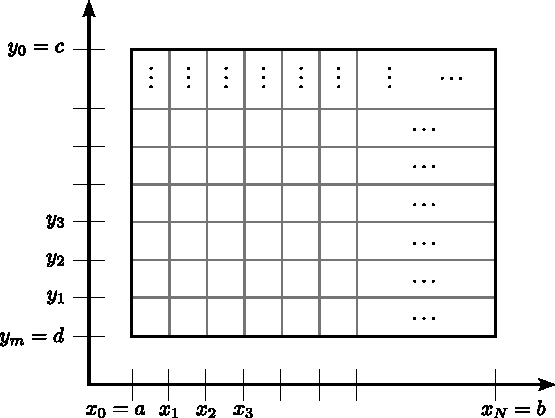
\includegraphics[scale=0.8]{figs/malla-01.pdf}
\end{center}
\cx
\textbf{Malla:}
\begin{itemize}
    \item División $[a, b]$ y $[c, d]$ en $n$ y $m$ partes iguales
    \item $h = (b - a) / n$, $k = (d - c) / m$
    \item $x_i = a + i h, \; i = 0, 1, \ldots, n$
    \item $y_j = c + j k, \; j = 0, 1, \ldots, m$
\end{itemize}

\textbf{Aproximación en diferencias finitas (serie de Taylor):}
\[ \frac{\partial^2 u}{\partial x^2} = \frac{u(x_{i+1}, y_j) - 2 u(x_i, y_j) + u(x_{i-1},y_j)}{h^2} + \bigO(h^2) \]
\[ \frac{\partial^2 u}{\partial y^2} = \frac{u(x_i, y_{j+1}) - 2 u(x_i, y_j) + u(x_i,y_{j-1})}{k^2} + \bigO(k^2) \]
\end{columns}
\end{frame}

\begin{frame}
    Con $u(x_i, y_j) \mapsto u_{i,j}$:
    \[ \frac{u_{i+1, j} - 2 u_{i,j} + u_{i-1, j}}{h^2} + \frac{u_{i, j+1} - 2 u_{i,j} + u_{i, j-1}}{k^2} = f_{i, j} + \frac{h^2}{12} \frac{\partial^4 u}{\partial x^4}(\xi_i, y_j) + \frac{k^2}{12} \frac{\partial^4 u}{\partial y^4}(x_i, \eta_j) \]
    para $i = 1, 2, \ldots, n-1$, $j = 1, 2, \ldots, m-1$ y condiciones de contorno:
\begin{align*}
    u_{0, j} &= g_{0, j} \txt{y} u_{n, j} = g_{n, j}, \quad j = 0, 1, \ldots m; \\
    u_{i, 0} &= g_{i, 0} \txt{y} u_{i, m} = g_{i, m}, \quad i = 0, 1, \ldots n
\end{align*}
Resulta:
\[ 2 \left[ \pow{\frac{h}{k}}{2} + 1 \right]  u_{i,j} - (u_{i+1, j} + u_{i-1,j}) - \pow{\frac{h}{k}}{2} (u_{i, j+1} + u_{i, j-1}) = -h^2 f_{i,j}, \; i \in [1, n-1], \; j \in [1, m-1] \]
\begin{columns}
\cx
    \begin{center}
        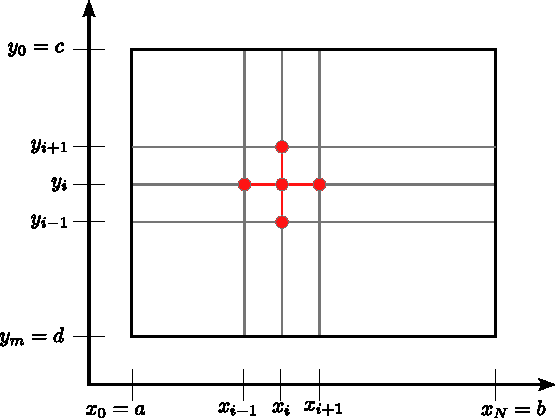
\includegraphics[scale=0.53]{figs/malla-02.pdf}
    \end{center}
\cx
\vspace{1em} \pause

\textbf{Ejemplo:} Determinar la distribución estacionaria de temperaturas en una placa de $0.5 \times 0.5$ m usando $n = m = 4$. Dos bordes adyacentes se mantienen a $0$ \textcelsius{} y la temperatura se incrementa linealmente en los otros bordes hasta llegar a $100$ \textcelsius{} en la esquina de unión.
\end{columns}
\end{frame}

\begin{frame}
\begin{columns}
\cx
\begin{center}
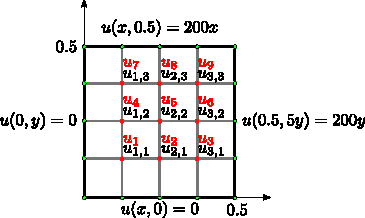
\includegraphics[scale=1.1]{figs/malla-03.pdf}
\end{center}

$u_{i,j} \mapsto u_l,\; l = i + m (j -1) $
\begin{align*}
    u_{1,1} &= u_1,\; u_{2,1} = u_2,\; u_{3,1} = u_{3} \\
    u_{1,2} &= u_4,\; u_{2,2} = u_5,\; u_{3,2} = u_{6} \\
    u_{1,3} &= u_7,\; u_{2,3} = u_8,\; u_{3,3} = u_{9} \\
\end{align*}
\cx
\[ \frac{\partial^2 u}{\partial x^2}(x, y) + \frac{\partial^2 u}{\partial y^2}(x, y) = 0; \;(x, y) \in [0, 0.5]^2 \]
\[ h = k = 1/8 \] \pause
Ecuaciones:
\[ 4 u_{i,j} - u_{i+1, j} - u_{i-1,j} -u_{i,j-1} -u_{i, j+1} = 0 \]
para $i = 1, 2, 3; \, j = 1, 2, 3$. \vspace{1em} \pause

Condiciones de borde:
\begin{align*}
    u_{0,0} &= u_{0,1} = u_{0,2} = u_{0,3} = u_{0, 4} = 0 \\
    u_{1,0} &= u_{2,0} = u_{3,0} = u_{4, 0} = 0 \\
    u_{1,4} &= u_{4,1} = 25; u_{2,4} = u_{4,2} = 50 \\
    u_{3,4} &= u_{4,3} = 75; u_{4,4} = 100
\end{align*}
\end{columns}
\end{frame}

\begin{frame}
\[
    \begin{bmatrix}
        4 & -1 & 0 & -1 & 0 & 0 & 0 & 0 & 0 \\
        -1 & 4 & -1 & 0 & -1 & 0 & 0 & 0 & 0  \\
        0 & -1 & 4 & 0 & 0 & -1 & 0 & 0 & 0  \\
        -1 & 0 & 0 & 4 & -1 & 0 & -1 & 0 & 0 \\
        0 & -1 & 0 & -1 & 4 & -1 & 0 & -1 & 0 \\
        0 & 0 & -1 & 0 & -1 & 4 & 0 & 0 & -1 \\
        0 & 0 & 0 & -1 & 0 & 0 & 4 & -1 & 0  \\
        0 & 0 & 0 & 0 & -1 & 0 & -1 & 4 & -1  \\
        0 & 0 & 0 & 0 & 0 & -1 & 0 & -1 & 4  \\
    \end{bmatrix}
    \begin{bmatrix} u_1 \\ u_2 \\ u_3 \\ u_4 \\ u_5 \\ u_6 \\ u_7 \\ u_8 \\ u_9 \end{bmatrix} = 
    \begin{bmatrix}
        u_{0,1} + u_{1,0} \\
        u_{0,2} \\
        u_{0,3} + u_{4,1} \\
        u_{0,2} \\
        0 \\
        u_{4,2} \\
        u_{0,3} + u_{1,4} \\
        u_{2,4} \\
        u_{3,4} + u_{3,4} \\
    \end{bmatrix} \rightarrow
    \begin{bmatrix} u_1 \\ u_2 \\ u_3 \\ u_4 \\ u_5 \\ u_6 \\ u_7 \\ u_8 \\ u_9 \end{bmatrix} = 
    \begin{bmatrix} 6.25 \\ 12.5 \\ 18.75 \\ 12.5 \\ 25 \\ 37.5 \\ 18.75 \\ 37.5 \\ 56.25 \end{bmatrix}
\] \pause

Solución exacta: $u(x, y) = 400 xy$ por lo que la aproximación en diferencias finitas no tiene error:
\[ \frac{\partial^4 u}{\partial x^4} = \frac{\partial^4 u}{\partial y^4} = 0 \]
\end{frame}

\begin{frame}
    \begin{columns}[t]
\cw{0.4}
Ecuación de calor (parabólica):
\[ \frac{\partial u}{\partial t} = \alpha \left(\frac{\partial^2 u}{\partial x^2} + \frac{\partial^2 u}{\partial y^2}\right) \] \pause
  \begin{center}
  \begin{overprint}
   \onslide<2-3>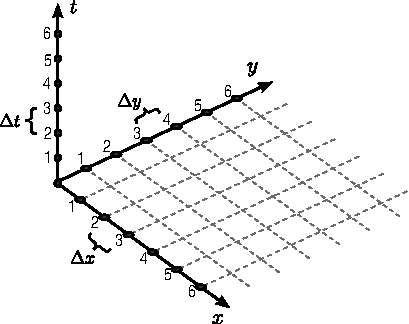
\includegraphics[width=1.0\textwidth]{figs/grilla}
   \onslide<4>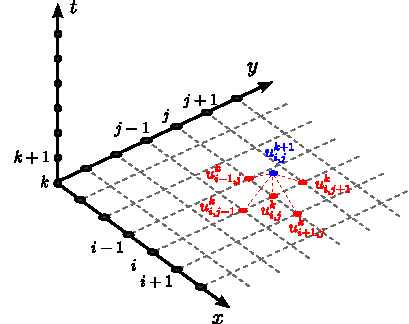
\includegraphics[width=1.0\textwidth]{figs/grilla-stencil}
  \end{overprint}
  \end{center}

\cw{0.6}
Grilla:
  \[ x_i = i \Delta x,\; y_j = j \Delta y,\; t_k = k \Delta t,\; u(x, y, t) = u_{i,j}^k\] \pause
  
  Diferencias finitas (hacia adelante - explícito):
  
  \begin{multline*} \frac{u_{i,j}^{k+1}-u_{i,j}^{k}}{\Delta t} = \alpha \left( \frac{u_{i+1,j}^{k} -2 u_{i,j}^{k}+u_{i-1,j}^{k}}{\Delta x^2} \right) \\
  + \left( \frac{u_{i,j+1}^{k} -2 u_{i,j}^{k}+u_{i,j-1}^{k}}{\Delta y^2} \right)
   \end{multline*}
  \pause

   Hacemos $\Delta x = \Delta y$, $\gamma = \alpha \dfrac{\Delta t}{\Delta x^2}$:
   \[ \textcolor{blue}{u_{i,j}^{k+1}} = \gamma \left( \textcolor{red}{u_{i+1,j}^{k}} + \textcolor{red}{u_{i-1,j}^{k}} + \textcolor{red}{u_{i,j+1}^{k}} + \textcolor{red}{u_{i,j-1}^{k}} - 4 \textcolor{red}{u_{i,j}^{k}} \right) + \textcolor{red}{u_{i,j}^{k}} \]
   
   Método explícito: $\Delta t \leq \dfrac{\Delta x^2}{4 \alpha}$ $\leftarrowtail $ estabilidad numérica.

\end{columns}
\end{frame}

\begin{frame}
    \begin{columns}
        \cw{0.4}
        \begin{center}
          \animategraphics[autoplay,loop, scale=0.6]{1}{figs/convolucion}{}{}
        \end{center}

        \cw{0.6}
        \alert{Stencil:}
   \[ \textcolor{blue}{u_{i,j}^{k+1}} = \gamma \left( \textcolor{red}{u_{i+1,j}^{k}} + \textcolor{red}{u_{i-1,j}^{k}} + \textcolor{red}{u_{i,j+1}^{k}} + \textcolor{red}{u_{i,j-1}^{k}} - 4 \textcolor{red}{u_{i,j}^{k}} \right) + \textcolor{red}{u_{i,j}^{k}} \]

    \end{columns}
\end{frame}

\begin{frame}
\begin{columns}
\cw{0.5}
   \[ \frac{\partial u}{\partial t} - \alpha \left( \frac{\partial^2 u}{\partial x^2} + \frac{\partial^2 u}{\partial y^2} \right) = 0 \]
   \[0 \leq x \leq L_x, \; 0 \leq y \leq L_y\]

 \begin{center}
 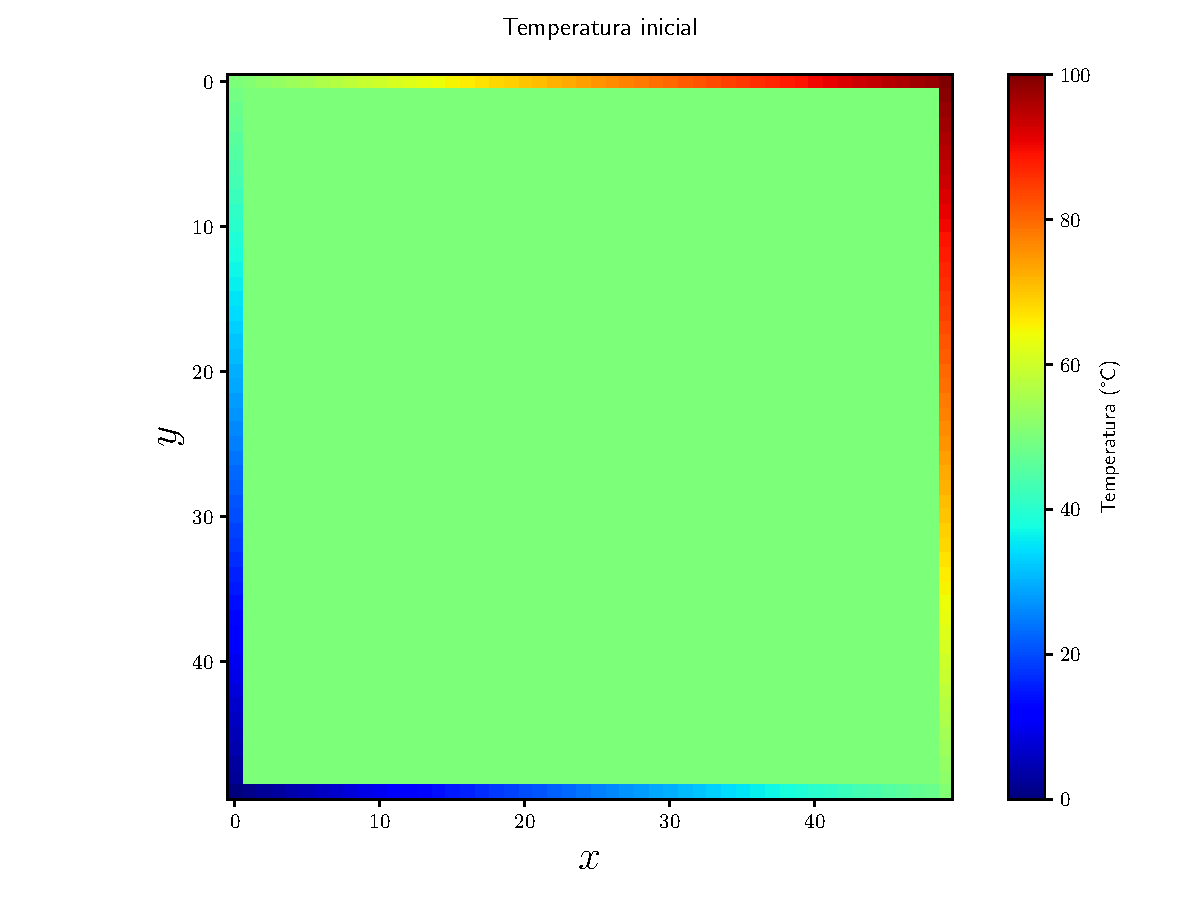
\includegraphics[width=1.0\textwidth]{code/temp-inicial.pdf}
\end{center}

\cw{0.5}
Condiciones de borde:
   \begin{align*}
       u(x, 0) &= 50 + \frac{x (100 - 50)}{L_x}  \\
       u(0, y) &= 50 - y \frac{50}{L_y} \\
    u(x, L_y) &= 50  \frac{x}{L_x} \\
    u(L_x, y) &= 100 - y \frac{50}{L_y} \\
   \end{align*}

Condición inicial:
\[ u(x, y)_{t=0} &= 50 \]
\end{columns}
\end{frame}

\begin{frame}
\begin{columns}
\cw{0.45}
\pycode[lastline=18]{code/ec-calor.py}
\cw{0.45}
\pycode[firstline=20, lastline=33]{code/ec-calor.py}
\begin{center}
    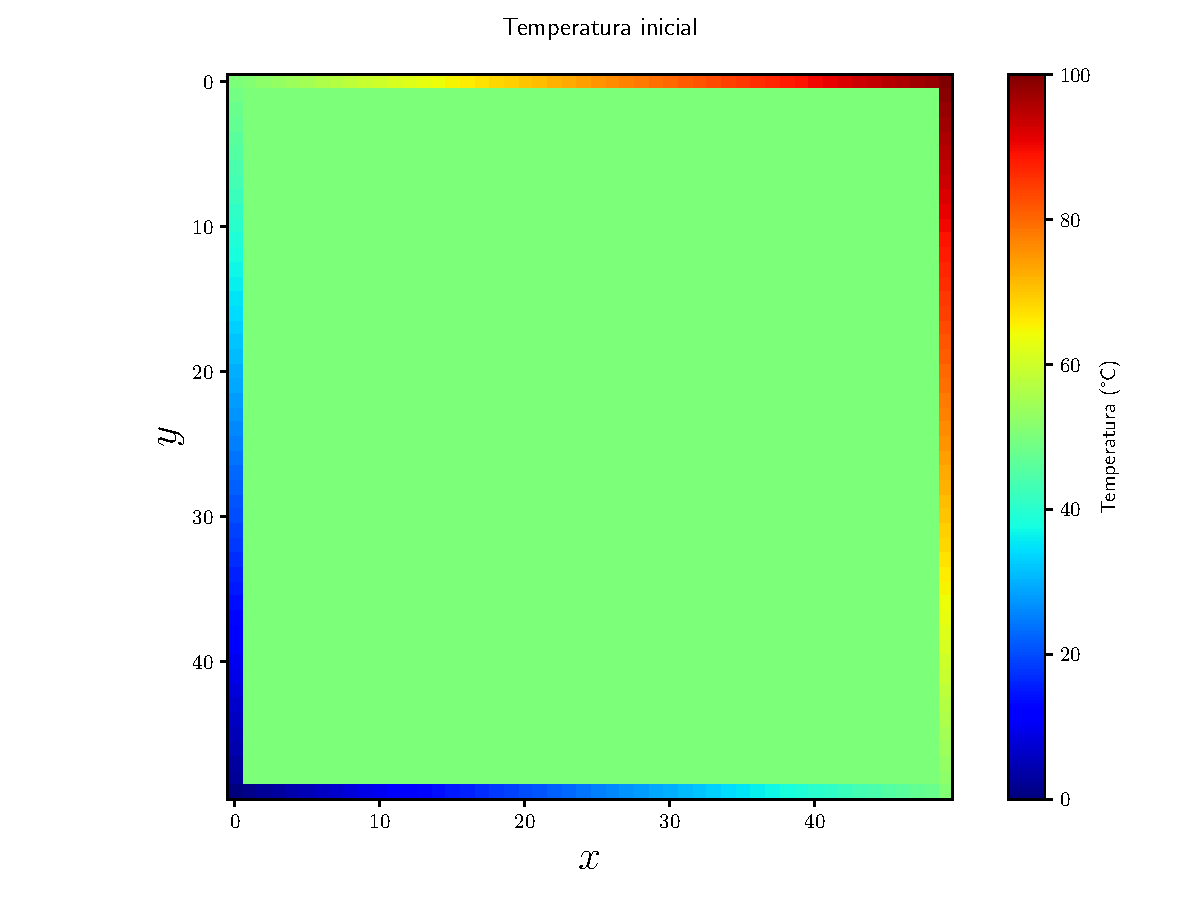
\includegraphics[width=0.7\textwidth]{code/temp-inicial.pdf}
\end{center}
\end{columns}
\end{frame}

\begin{frame}
\begin{columns}
\cw{0.45}
\pycode[firstline=35, lastline=47]{code/ec-calor.py}
\cw{0.45}
\pycode[firstline=49, lastline=60]{code/ec-calor.py}
\begin{center}
    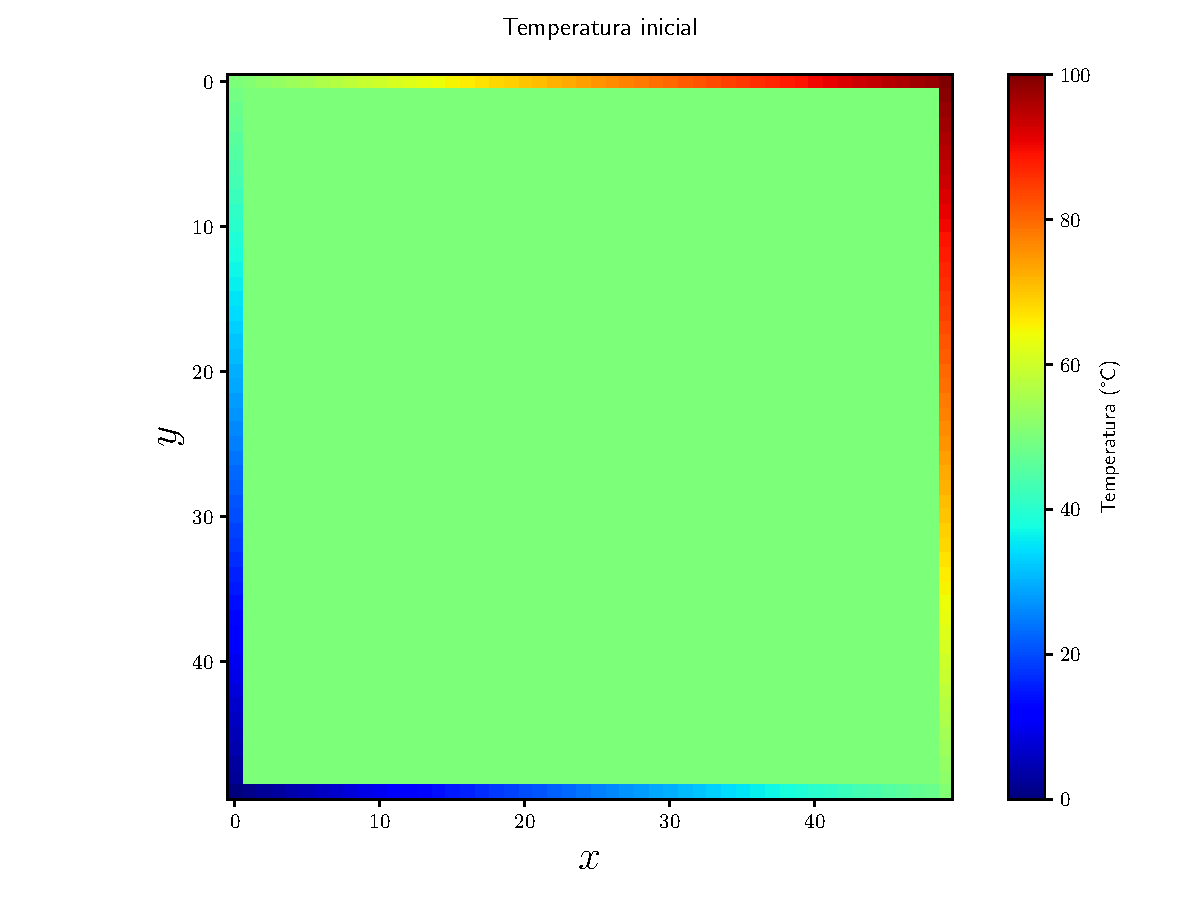
\includegraphics[width=0.7\textwidth]{code/temp-inicial.pdf}
\end{center}
\end{columns}
\end{frame}

\begin{frame}
\begin{columns}
\cw{0.6}
\pycode[firstline=49, lastline=70]{code/ec-calor.py}

\cw{0.38}
\begin{center}
    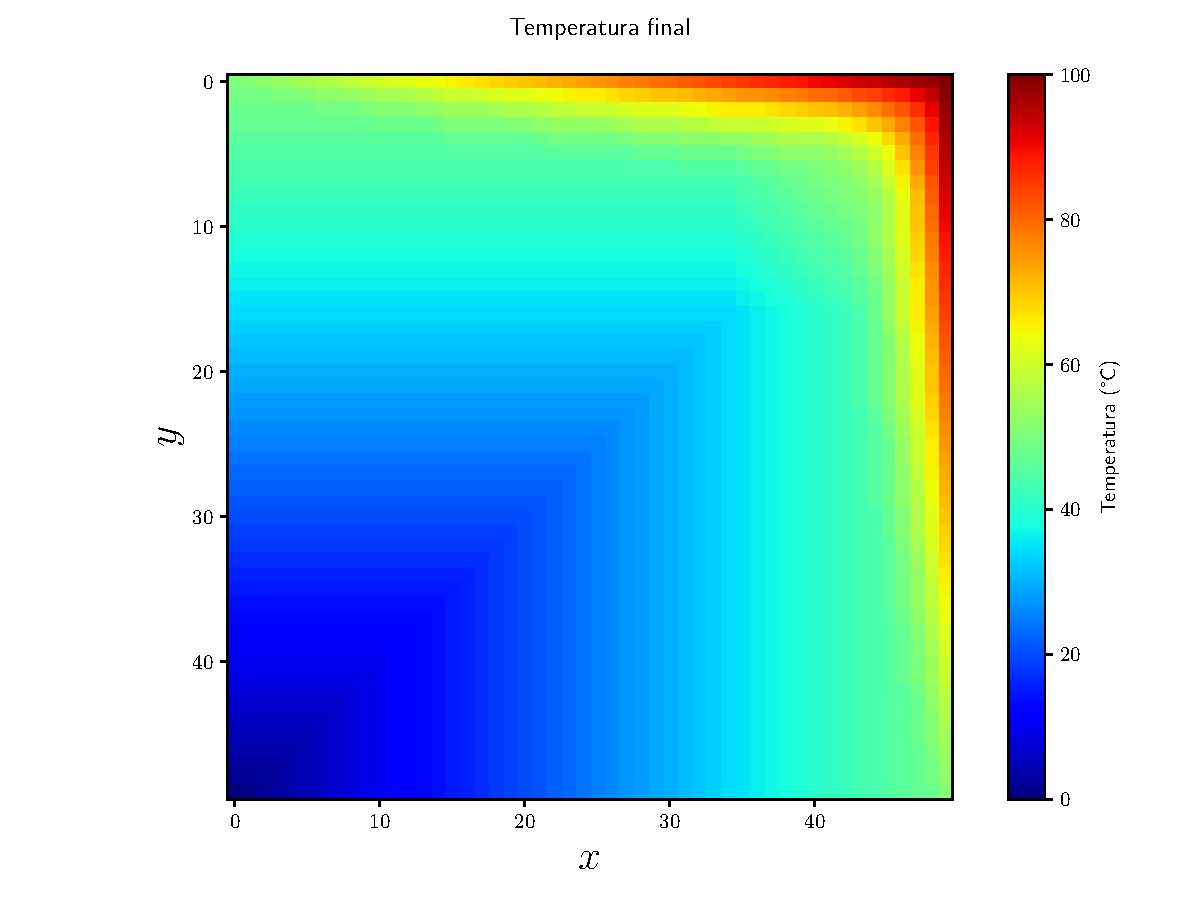
\includegraphics[width=1.0\textwidth]{code/temp-final.pdf}
\end{center}
\end{columns}
\end{frame}

\begin{frame}
\begin{columns}
\cw{0.45}
\pycode[firstline=72, lastline=96]{code/ec-calor.py}
\pause

\cw{0.45}
\begin{center}
 \embedvideo{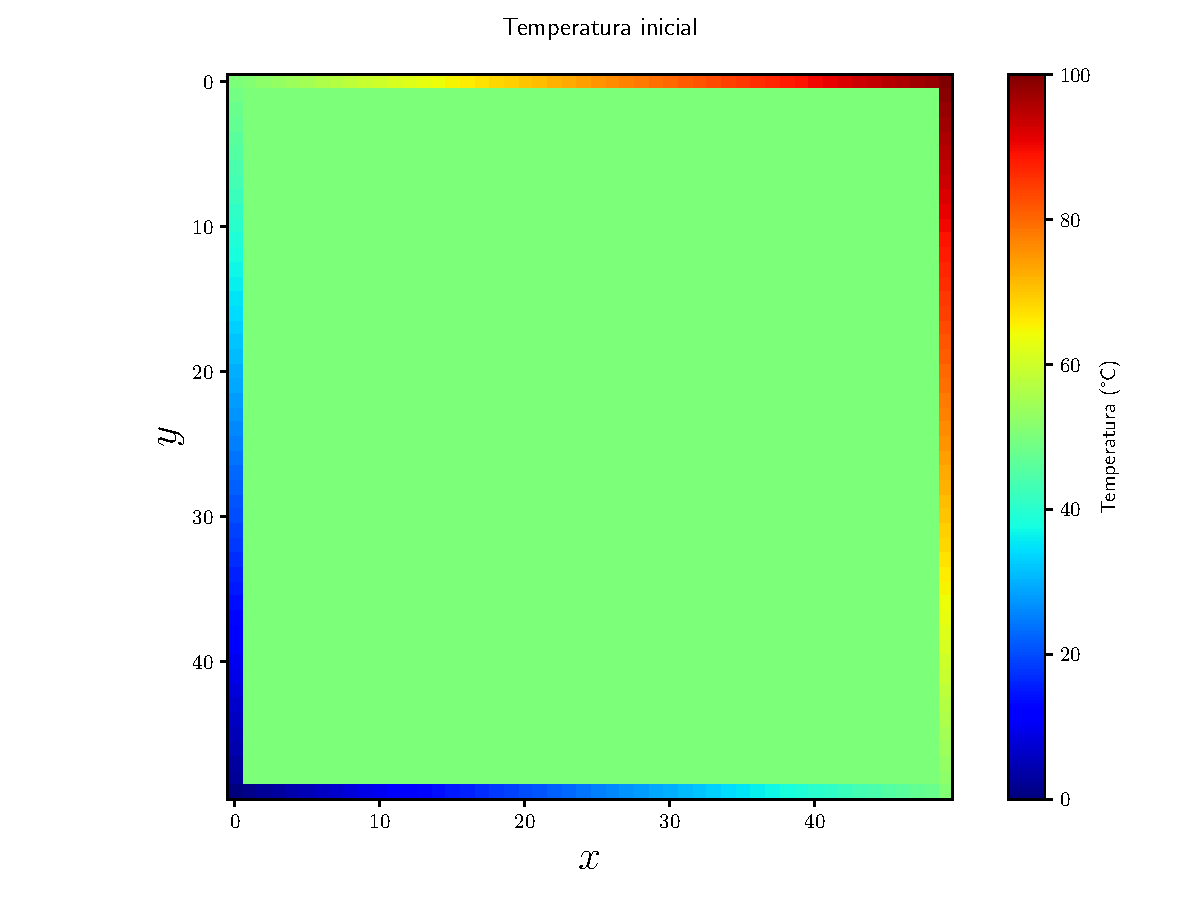
\includegraphics[width=1.0\textwidth]{code/temp-inicial.pdf}}{code/solucion_ecuacion_calor_t.mp4} 
 \end{center}
\end{columns}
\end{frame}

%% Esquema implícito y Crank-Nicolson en Burden 12.2


\section*{Bibliografía}
\begin{frame}[allowframebreaks]{Lecturas recomendadas}
\begin{itemize}
    \item \fullcite{burden2017}. Capítulo 12.
\item \fullcite{kreyszig2011}. Capítulo 21.
    \item \fullcite{langtangenLinge2016}. Capítulo 3.
\end{itemize}
\end{frame}

\end{document}

